\chapter[Capturing Concentration-Induced Aggregation of Nucleobases on a Graphene Surface through Polarizable Force Field Simulations]{Capturing Concentration-Induced Aggregation of Nucleobases on a Graphene Surface through Polarizable Force Field Simulations \protect\footnote[3]{This chapter has been published as \textbf{H., Hemanth}, Yadav, P. K. and Mallajosyula*, S.S.; Capturing Concentration Induced Aggregation of Nucleobases on Graphene Surface Through Polarizable Forcefield Simulations; {\textit{J. Phys. Chem. C}, 2022, \textbf{31}, 13122 - 13131}}}
\section{Introduction}
Controlled supramolecular assemblies formed by small molecules on two-dimensional (2D) supports have attracted significant attention in the scientific community.\supercite{goronzy_supramolecular_2018, moradi_two-dimensional_2017,quesne-turin_first-principles_2017} Noncovalent interactions such as hydrogen bonding, $\pi$-$\pi$ stacking, and electrostatic interactions play a fundamental role in stabilizing such supra-molecular assemblies.\supercite{subramani_self-assembly_2012} Here, nucleobases offer a viable pathway to the realization of both structured and amorphous self-assemblies due to the presence of multiple hydrogen bond donors and acceptors.\supercite{saravanan_surface_2018, saikia_hierarchical_2017, freund_structure_1997, heckl_two-dimensional_1991, saikia_dynamics_2018, kelly_understanding_2008, lukas_adenine_2009, wandlowski_structure_1996, otero_elementary_2008}. Chemical moieties with a nucleobase core act as starting blocks for rosette nanotubes\supercite{marsh_self-complementary_1996, fenniri_helical_2001} and other self-assemblies.\supercite{lafitte_quadruply_2006, park_highly_2005, sessler_novel_2003} Self-assemblies formed by nucleobases or their derivatives have found applications in bionanotechnology\supercite{laguerre_synthetic_2015, suri_role_2009, song_self-assembled_2011} and catalysis.\supercite{chhabra_electroless_2011, borzsonyi_water-soluble_2010} A fundamental understanding of the behavior of nucleobases at the solid-liquid interface is also crucial in understanding the evolution of life from simple chemical moieties.\supercite{cassidy_guanine-centric_2014, sowerby_role_1998}

Cytosine, one of the five natural nucleobases, can spontaneously self-assemble into higher-order structures over various solid-state supports such as Au(111),\supercite{kelly_understanding_2008, otero_elementary_2008} Cu(111)\supercite{tanaka_two-dimensional_1996} and highly oriented pyrolytic graphite (HOPG).\supercite{xu_directional_2021} Electroanalytical studies coupled with in situ STM imaging by Wandloski et al. showed that cytosine self-assemblies respond to an external voltage.\supercite{wandlowski_structure_1996} Otero et al. studied the formation of self-assembled networks in cytosine adsorbed over a Au(111) surface.\supercite{otero_elementary_2008} They observed the formation of geometries like five-/six-membered rings and filaments, which exist as a part of a more extensive self-assembled random network; 2D structures like graphene provide unique solid-state supports that are truly atomistically thin, as compared to the solid-state supports like Au(111) and Cu(111) surfaces. It is of interest to explore if graphene as a support can exhibit self-assembly properties akin to the metallic solid-state supports.

Molecular dynamics (MD) simulations provide a computational framework to gain insight into the atomistic interactions involved in the interfacial phenomenon. MD simulations have been used to study the self-assembly of nucleobases and other small molecules on solid-state supports like Au(111),\supercite{rapino_modeling_2005, maleki_molecular_2011, rosa_enthalpyentropy_2014} \textit{h}-BN,\supercite{ding_adsorption_2013, saikia_polarity-induced_2018} graphene,\supercite{saikia_hierarchical_2017, saikia_dynamics_2018} C\textsubscript{2}N,\supercite{mukhopadhyay_gauging_2018, mukhopadhyay_screening_2020} g-C\textsubscript{3}N\textsubscript{4},\supercite{mukhopadhyay_delicate_2020} and black-PN.\supercite{mukhopadhyay_design_2018}  However, it has been found that simulations using additive force fields (FF) do not capture the self-assembly behavior of nucleobases on 2D supports, rather the simulations capture a dispersive behavior for nucleobases adsorbed over the graphene sheet.\supercite{saikia_dynamics_2018} Tekin et al. reported that a modified Buckingham potential could capture the self-assembly of cytosine until hexamers in MD simulations.\supercite{manukyan_first_2015} However, specialized potentials, like the ones developed by Tekin et al., might not be immediately transferable to systems containing biomolecular entities. Having a FF that captures both the aggregation dynamics of nucleobases and is readily compatible with other components of the simulation system is desirable to ensure the continued applicability of MD simulations to such problems. We have recently shown that MD simulations based on the Drude polarizable FF could accurately capture higher-order structures in cytosine molecules adsorbed on a graphene sheet.\supercite{h_polarization_2021} In our work we established that inclusion of polarization captured the $\pi$-$\pi$ stacking as well as hydrogen-bonded network formation, while additive simulations only resulted in random dispersion of nucleobases on the 2D graphene support. We refer the reader to an earlier work for a detailed comparison between the additive and polarizable simulations.\supercite{h_polarization_2021} We showed that cytosine molecules adsorbed onto the graphene sheet self-assembled into C1-D(2) ribbon type structures previously observed by Kelly et al. via STM imaging and DFT calculations.\supercite{kelly_understanding_2008}

Self-assembly studies are generally hampered by the formation of solution aggregate structures as opposed to the desirable uniformly dispersed monolayer self-assembly on the underlying solid-state support.\supercite{lotito_approaches_2017} The balance between solution aggregation and solid-supported monolayer formation is generally dependent on the concentration of the solute. In the present study, we investigate the effect of concentration on the adsorption dynamics and self-assembly of nucleobases in the presence of graphene as a solid support. To this end, we study the dynamics of cytosine nucleobases dispersed on the graphene sheet at three different concentrations 0.25 M (21 nucleobases), 0.50 M (45 nucleobases), and 0.75 M (60 nucleobases). The study reveals the dependence of concentration and the interplay of intermolecular nonbonded interactions, hydrogen bonding, and $\pi$-$\pi$ interactions, controlling the formation of the observed structures.

\section{Computational Methodology}
Graphene sheets, with a radius of 21 $\angstrom$ and height of 2 $\angstrom$, were constructed using Inorganic Builder Toolkit available in VMD.\supercite{humphrey_vmd_1996} We used two graphene sheets separated by 55 $\angstrom$ to model the graphene surface. The molecular geometries of cytosine nucleobases were generated utilizing the topology information present in the Chemistry at Harvard Molecular Mechanics (CHARMM) additive nucleic acid FF\supercite{hart_optimization_2012, foloppe_all-atom_2000, mackerell_all-atom_2000} (CHARMM36) using the CHARMM program.\supercite{brooks_charmm_1983, brooks_charmm_2009} On the basis of the concentration, 21 nucleobases (0.25 M), 45 nucleobases (0.50 M), and 60 nucleobases (0.75 M) were added to the system. The nucleobases were initially arranged as an ordered matrix, with the interplanar distances set to 7 $\angstrom$ in all three dimensions, in an attempt to avoid biasing the system toward intermolecular $\pi$-stacking interactions. The layer closest to the graphene sheet in the cytosine matrix was placed at least 10 $\angstrom$ above the graphene sheet to avoid self-assembly bias. The nucleobase - graphene system was solvated using VMD to bring the system dimensions to (52 × 52 × 60) $\angstrom$\textsuperscript{3} The Drude particles were added to the final solvated systems using in-house scripts. In Figure 4.1, we present the representative structure depicting the system setup.

\begin{figure}
    \centering
    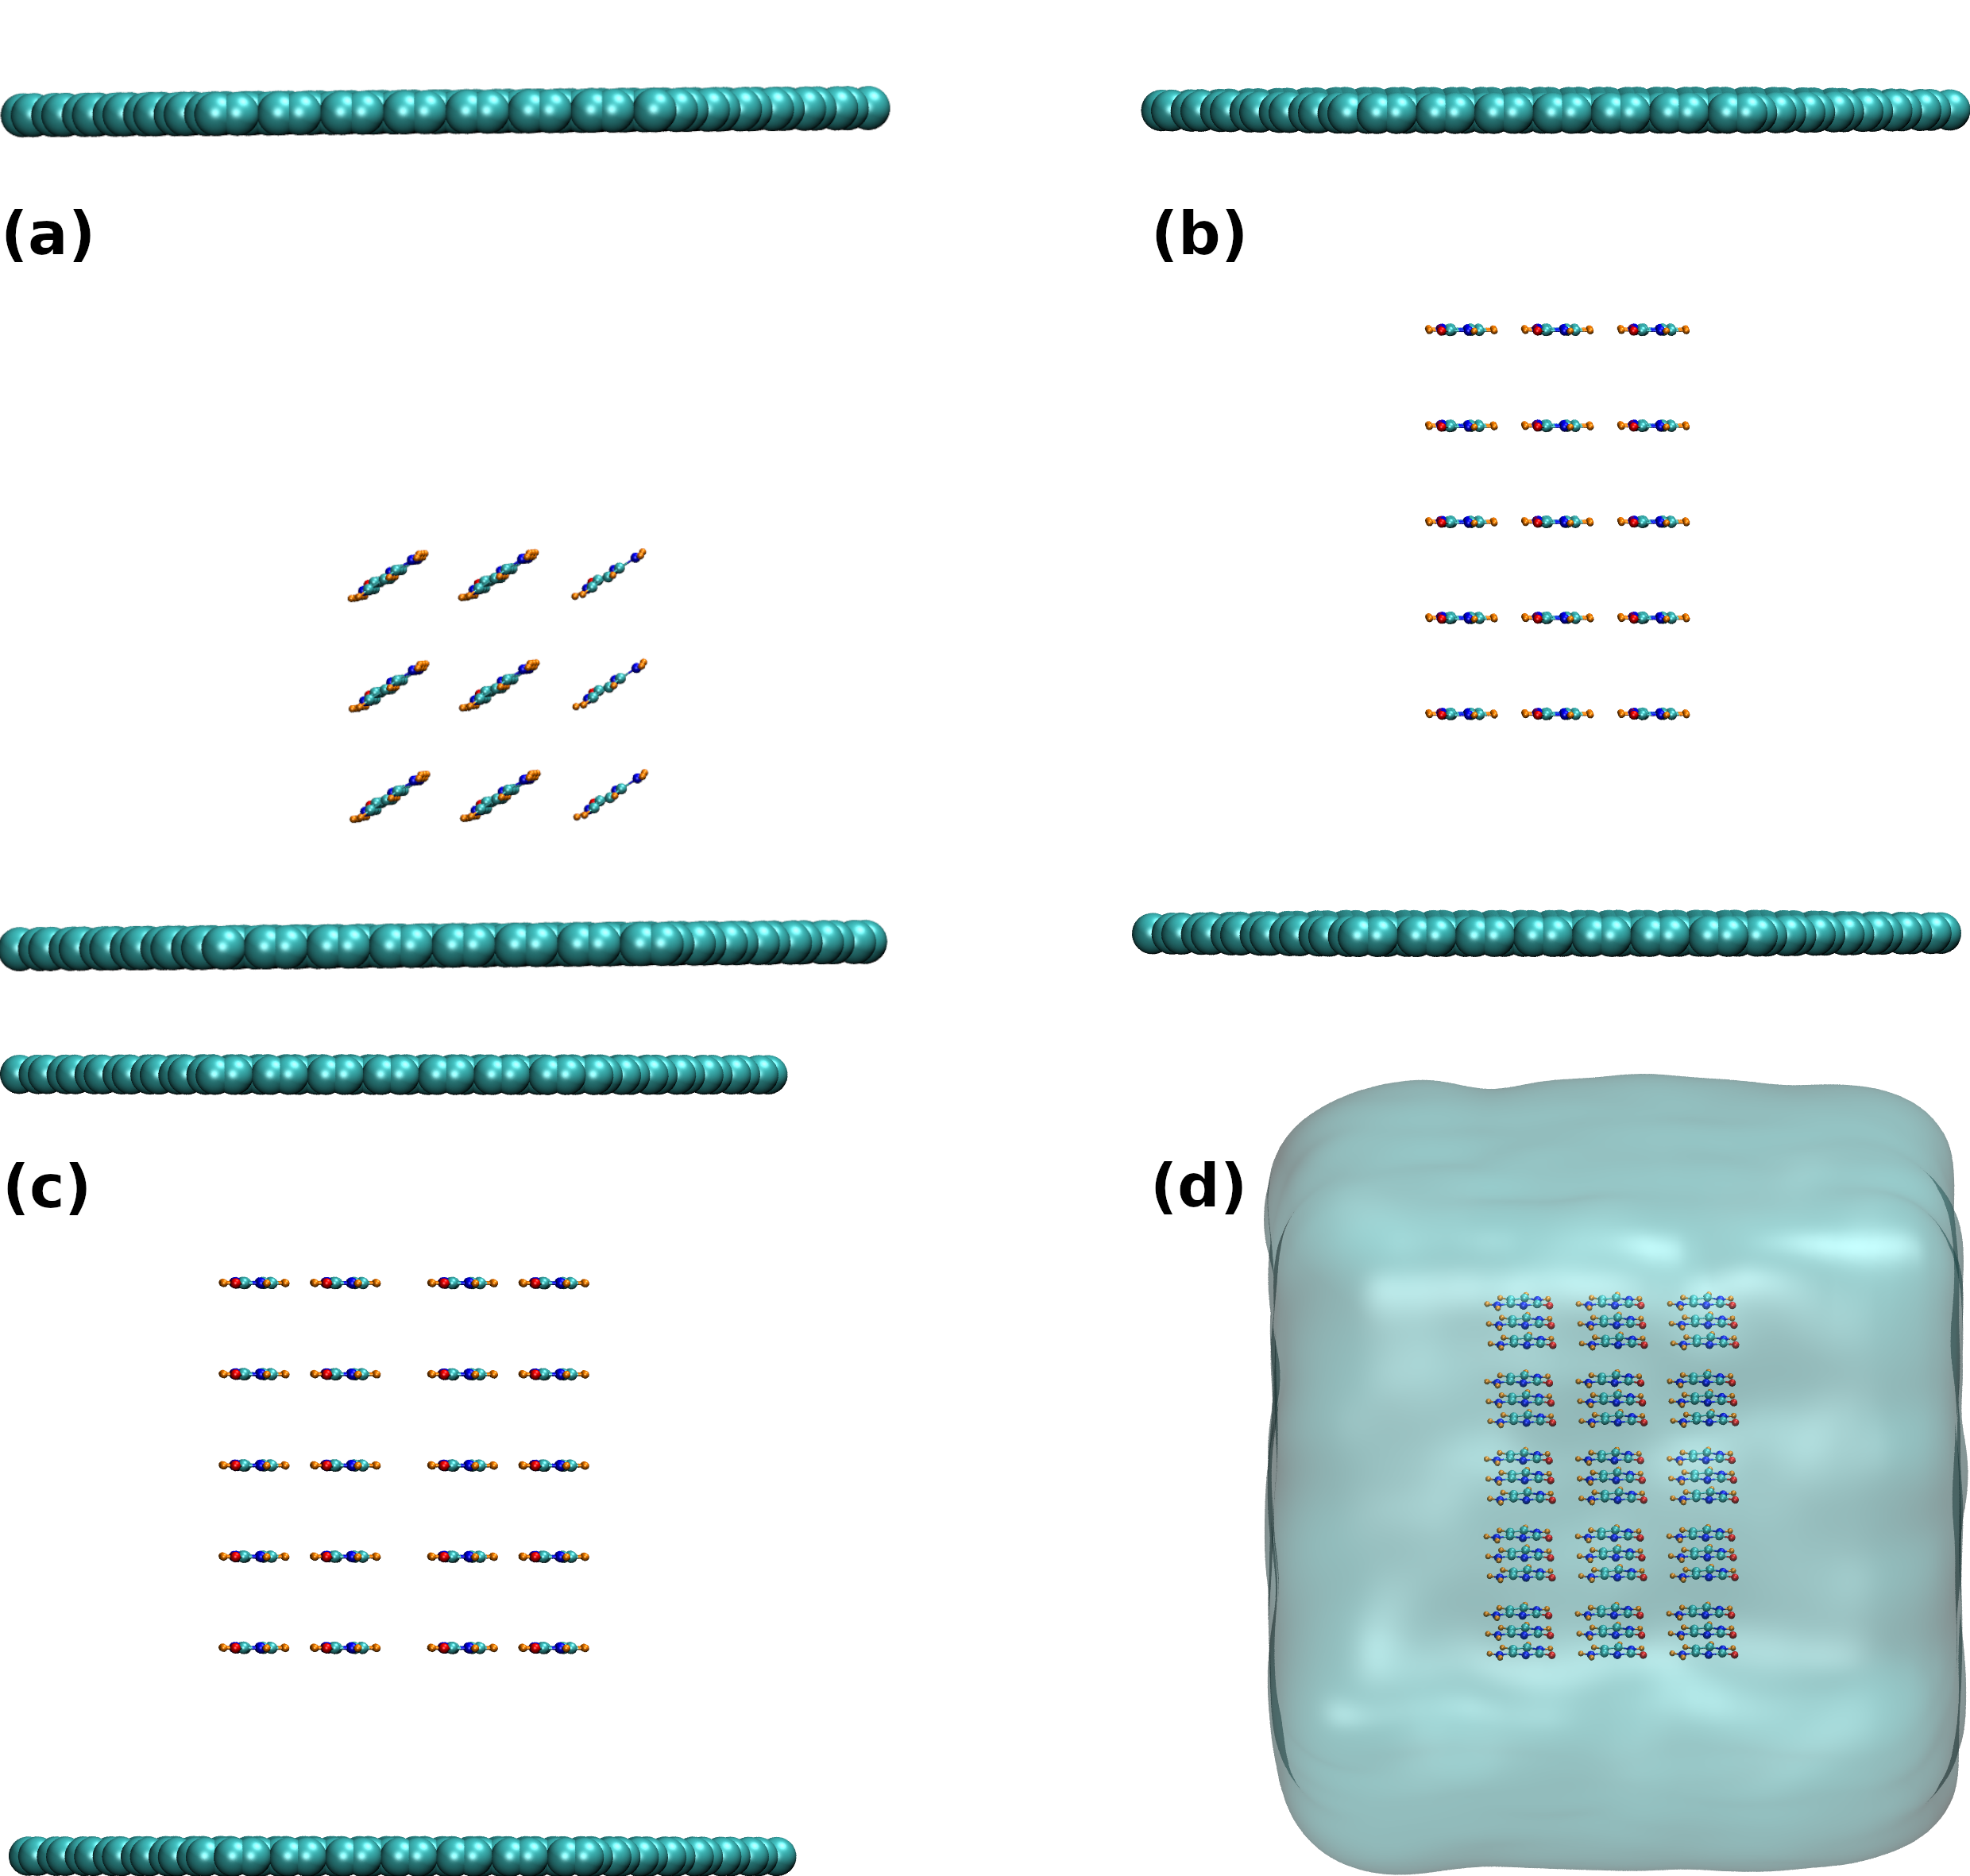
\includegraphics{Chapter2/Figures/Figure0.png}
    \caption[Representative structures of the initial system setup for various systems investigated in this paper]{Representative structures of the initial system setup for (a) 0.25M, (b) 0.50M, (c) 0.75M nucleobase - graphene, and (d) 0.60M freestanding nucleobase simulations. Carbon atoms are coloured green, nitrogen atoms are blue, oxygen atoms are red and hydrogen atoms are orange. Water molecules have been excluded from (a), (b) and (c) for clarity}
\end{figure}

The MD simulations were performed in the isobaric-isothermal (NPT) ensemble using the Nanoscale Molecular Dynamics (NAMD) simulation package.\supercite{phillips_scalable_2005} The Classical Drude polarizable FF was used to describe the bonded and nonbonded interactions of the nucleobases. Classical Drude polarizable parameters previously tested by us for studying graphene - nucleobase interactions\supercite{h_polarization_2021} were used to describe the bonded and nonbonded interactions of the graphene sheet. Water molecules were described by SWM4-NDP polarizable water model\supercite{lamoureux_polarizable_2006} with bond lengths and bond angles constrained via the SETTLE\supercite{miyamoto_settle_1992} algorithm. Particle Mesh Ewald (PME) summation\supercite{darden_particle_1993} was used to evaluate electrostatic interactions with a cutoff of 9.0 $\angstrom$. All simulations were performed at room temperature (298 K) with Langevin dynamics and a Nos\'{e}-Hoover Langevin piston applied to maintain the pressure at 1 atm. An additional dual thermostat was applied to maintain the Drude particles in an ice bath at 1 K.

The nucleobase - graphene systems were minimized for 60000 steps using conjugate-gradient (CG) minimization to remove unfavorable contacts. Minimized structures were equilibrated in an NPT ensemble for 1 ns. The central atom of the graphene sheet was constrained using a harmonic potential of 1.0 kcal (mol $\angstrom$)\textsuperscript{-2} to ensure that the sheets did not slide during the simulations. No additional constraints were applied, with the sheets allowed to ``breathe'' over the course of the simulations. The equations of motion were integrated using a time step of 1 fs. Production simulations were carried out for 750 ns for all the nucleobase - graphene systems, except for the 0.75 M system which was run for 600 ns. 

To estimate the influence of the graphene surface on the aggregation dynamics of cytosine nucleobases we also simulated cytosine nucleobases in water. A 0.60 M system of cytosine nucleobases in a water box of dimensions (50 × 50 × 50) $\angstrom$\textsuperscript{3} was generated using CHARMM and VMD. A total of 45 nucleobases were arranged in an ordered matrix, with interplanar distances set to 7 $\angstrom$ in all dimensions to prevent the system from biasing toward intermolecular $\pi$-stacking interactions. The Drude particles were added to the final solvated system using in-house scripts. A representative image showing the system setup is presented in Figure 4.1. The system was minimized for 60000 steps using CG minimization and subsequently equilibrated in an isobaric-isothermal ensemble for 1 ns. Production simulations were carried out for 500 ns. The same simulation parameters as described earlier were used for studying the cytosine nucleobase water simulation.

Plugins available in VMD were used to analyze hydrogen bonds and instantaneous dipole moment of the nucleobases. In-house analysis scripts were used for analyzing the formation of $\pi$-stacks, hydrogen-bonded networks, and the relative orientation of the nucleobases.

\section{Results and Discussions}
In our earlier study, we observed that at low concentrations (0.25 M) the cytosine nucleobases formed a well-dispersed monolayer on the graphene sheet. This was characterized by analyzing two collective variables: (1) projected distance between the center-of-mass (COM) of the nucleobase and graphene sheet (d\textsubscript{Nuc-Graph}) and (2) relative orientation of the nucleobase with respect to the graphene sheet ($\theta$\textsubscript{Nuc-Graph}). In Figure 4.2, we illustrate the collective variables employed to track the interaction of nucleobases with the underlying graphene sheet.
In Figure B.1 of the Appendix B, we present the time series corresponding to d\textsubscript{Nuc-Graph} obtained from the 0.25, 0.50, and 0.75 M simulations. We observe that fluctuations in the d\textsubscript{Nuc-Graph} time series cease beyond 250 ns for the 0.25 and 0.50 M simulations, indicative of the systems reaching an equilibrium. For the 0.75 M simulations, the simulations are deemed convergent after first 100 ns, wherein the fluctuations in the d\textsubscript{Nuc-Graph} time series cease, denoting the equilibrium state.  In the remainder of the chapter, the last 500 ns of the simulation trajectories are used for analysis. In Figure B.2 of the Appendix B, we present the probability distribution corresponding to d\textsubscript{Nuc-Graph} evaluated for two blocks of the simulation trajectory, 250-500 ns and 500-750 ns, for the 0.25 and 0.50 M simulations. For the 0.75 M simulation, we present the probability distribution for blocks corresponding to 100-350 ns and 350-600 ns. We observe significant overlap between the distributions.
\begin{figure}
    \centering
    \includegraphics{Chapter2/Figures/Figure1.png}
    \caption[Representative illustration of collective variables used to study the evolution of nucleobase - graphene simulations]{Representative illustration of collective variables used to study the evolution of nucleobase - graphene simulations. (a) d\textsubscript{Nuc-Graph} and (b) $\theta$\textsubscript{Nuc-Graph}. d\textsubscript{Nuc-Graph} is calculated as the difference between the z-coordinates of the COM of nucleobase and top layer of the graphene sheet. $\theta$\textsubscript{Nuc-Graph} is calculated as \textit{arccos(Normal.z-axis)}.}
\end{figure}

\begin{figure}
    \centering
    \includegraphics[width=\textwidth]{Chapter2/Figures/Figure2.png}
    \caption[Probability distribution of d\textsubscript{Nuc-Graph} and $\theta$\textsubscript{Nuc-Graph} for cytosine nucleobases at 0.25, 0.50, and 0.75 M, respectively. Representative structures corresponding to identified features are also presented]{Probability distribution of (a) d\textsubscript{Nuc-Graph} for cytosine nucleobases at 0.25, 0.50, and 0.75 M, respectively. (b) Representative image of the 0.25 M simulations, (c) Probability distribution of $\theta$\textsubscript{Nuc-Graph} for cytosine nucleobases at 0.25, 0.50, and 0.75 M, respectively. (d) $\theta$\textsubscript{Nuc-Graph} distribution as a function of d\textsubscript{Nuc-Graph} distance for 0.50 M simulations. (e) Representative image of the 0.50 M simulations, nucleobases in regions (i) (d\textsubscript{Nuc-Graph} < 4.5 $\angstrom$), (ii) (4.5 $\angstrom$ < d\textsubscript{Nuc-Graph} < 8.5 $\angstrom$), and (iii) (d\textsubscript{Nuc-Graph} > 8.5 $\angstrom$) are presented in red, blue, and green, respectively. (f) $\theta$\textsubscript{Nuc-Graph} distribution as a function of d\textsubscript{Nuc-Graph} distance for 0.75 M simulations. (g) Representative image of the 0.75 M simulations; color coding is similar to the representative image for 0.50 M simulations. Distances are presented in $\angstrom$ and orientations are presented in degrees (deg).}
\end{figure}
In Figure 4.3(a), we present the probability distribution corresponding to d\textsubscript{Nuc-Graph} for all the systems. For the 0.25 M simulations, we observe a single peak in the d\textsubscript{Nuc-Graph} distribution at a distance of 3.5 $\angstrom$ that is indicative of the formation of a monolayer of nucleobases on the graphene sheet [Figure 4.3(a)]. In Figure 4.3(b), we present a representative snapshot of the arrangement of the nucleobases on the graphene sheet from the 0.25 M simulations. In Figure 4.3(c), we present the probability distribution corresponding to $\theta$\textsubscript{Nuc-Graph} for all the systems. For the 0.25 M simulations, we observe that the formation of this monolayer is driven by the $\pi$-$\pi$ interactions between the nucleobase and the underlying graphene sheet. This observation is consistent with our earlier studies\supercite{h_polarization_2021} and the results previously reported by Saikia et al., where cytosine nucleobases were found to tile the surface of the graphene sheet.\supercite{saikia_dynamics_2018} The fact that the nucleobases lie flat on the graphene sheet is also corroborated by the $\theta$\textsubscript{Nuc-Graph} bimodal distribution for 0.25 M simulations with 175$\degree$ < $\theta$\textsubscript{Nuc-Graph} < 5$\degree$ [Figure 4.3(c)]. For 0.50 M simulations, we observe multiple peaks in the d\textsubscript{Nuc-Graph} distribution at around 3.5, 7.0, 10.5, and 14.0 $\angstrom$ [Figure 4.3(a)]. The peaks at 3.5 and 7.0 $\angstrom$ appear as sharp distributions, while the peaks at 10.5 and 14.0 $\angstrom$ appear as broad distributions. Analyzing the molecular interactions giving rise to these distributions, we observe that the peaks at 3.5 and 7.0 $\angstrom$ correspond to the formation of a monolayer assembly of the cytosine nucleobases. This is corroborated by analyzing the $\theta$\textsubscript{Nuc-Graph} distribution relative to the d\textsubscript{Nuc-Graph} distances presented in Figure 4.3(d). The $\theta$\textsubscript{Nuc-Graph} distribution is analyzed for three regions: (i) d\textsubscript{Nuc-Graph} < 4.5 $\angstrom$, (ii) 4.5 $\angstrom$ < d\textsubscript{Nuc-Graph} < 8.5 $\angstrom$, and (iii) d\textsubscript{Nuc-Graph} > 8.5 $\angstrom$. Regions (i) and (ii) correspond to the peaks at 3.5 and 7.0 $\angstrom$, while region (iii) corresponds to the broad distributions around 10.5 and 14.0 $\angstrom$. For both regions (i) and (ii), we observe a bimodal $\theta$\textsubscript{Nuc-Graph} distribution with 175$\degree$ < $\theta$\textsubscript{Nuc-Graph} < 5$\degree$, indicating that in both the distributions the nucleobases lie flat relative to the underlying graphene sheet. Thus, the monolayer at 3.5 $\angstrom$ is stabilized by $\pi$-$\pi$ interactions between the nucleobase and the underlying graphene sheet, while the monolayer at 7.0 $\angstrom$ is stabilized by $\pi$-$\pi$ interactions between the cytosine nucleobases in the first monolayer and the second monolayer. For region (iii), corresponding to nucleobases beyond 8.5 $\angstrom$, we observe a continuous distribution for $\theta$\textsubscript{Nuc-Graph} as opposed to the bimodal distribution observed for regions (i) and (ii). Both d\textsubscript{Nuc-Graph} and $\theta$\textsubscript{Nuc-Graph} indicate a disruption of the $\pi$-stacked monolayer structure beyond 8.5 $\angstrom$. This is due to nucleobase - nucleobase aggregation that is stabilized via intermolecular hydrogen bonding and $\pi$-$\pi$ interactions. In Figure 4.3(e), we present a representative snapshot from the 0.50 M simulation illustrating the arrangement of the nucleobases in the three regions as defined by the d\textsubscript{Nuc-Graph} distribution. Upon increasing the concentration to 0.75 M, we observe the formation of three distinct peaks in the d\textsubscript{Nuc-Graph} distribution, centered at 3.5, 7.0, and 10.5 $\angstrom$ [Figure 4.3(a)]. It is observed that the peak at 3.5 $\angstrom$ has a sharp feature, while the peaks at 7.0 and 10.5 $\angstrom$ appear as broad distributions. We analyze the $\theta$\textsubscript{Nuc-Graph} distribution for three regions: (i) d\textsubscript{Nuc-Graph} $\leq$ 4.5 $\angstrom$, (ii) 4.5 < d\textsubscript{Nuc-Graph} $\leq$ 8.5 $\angstrom$, and (iii) d\textsubscript{Nuc-Graph} > 8.5 $\angstrom$. The resulting distributions are presented in Figure 4.3(f). Nucleobases lying in the region d\textsubscript{Nuc-Graph} $\leq$ 4.5 $\angstrom$ lie flat on the graphene sheet, which is corroborated by the bimodal distribution of $\theta$\textsubscript{Nuc-Graph} with peaks centered at < $\theta$\textsubscript{Nuc-Graph} = 175$\degree$ and $\theta$\textsubscript{Nuc-Graph} = 5$\degree$. Thus, the nucleobases closest to the graphene sheet form a monolayer assembly stabilized by $\pi$-$\pi$ interactions between the nucleobases and underlying graphene sheet. For nucleobases lying in regions (ii) and (iii), we observe that $\theta$\textsubscript{Nuc-Graph} adopts a broad distribution, indicative of the formation of nucleobase aggregates, which are stabilized by intermolecular hydrogen bonding and $\pi$-$\pi$ interactions.
\begin{figure}
    \centering
    \includegraphics[width=\textwidth]{Chapter2/Figures/Figure3.png}
    \caption[Probability distributions of anngle between the normal ($\phi$) of the nucleobases involved $\pi$-stacks and hydrogen-bonded dimers. Representative structures corresponding to identified features are also presented.]{(a) Representative image from the 0.60 M nucleobase simulations. Hydrogen bonds are illustrated by dotted lines. (b) Probability distribution of the angle between the normal ($\phi$) of the nucleobases involved in $\pi$-stacks. Representative images illustrating the side-view and top-view of the antiparallel and parallel arrangement of the $\pi$-stacks corresponding to $\phi$ values of 42 and 138$\degree$. (c) Probability distribution of the angle between the normal ($\phi$) of the nucleobases involved in hydrogen-bonded dimers. Representative images illustrating the arrangement of the nucleobases corresponding to the peaks in the distribution.}
\end{figure}

\begin{figure}
    \centering
    \includegraphics[width=\textwidth]{Chapter2/Figures/B3_port.png}
    \caption[Time series plots for number of $\pi$-stacks and hydrogen - bonded dimers in 0.60M simulations]{Time series plots for number of (a) $\pi$-stacks and (b) hydrogen - bonded dimers in 0.60M simulations.}    
\end{figure}

To comment on the aggregate structures, we analyze the solution structures obtained from the 0.60 M nucleobase-only simulations. In Figure 4.4(a), we present a representative snapshot obtained from the nucleobase only simulations. We observe aggregate formations which are stabilized by $\pi$-$\pi$ interactions and intermolecular hydrogen bonding. To quantify the $\pi$-stacked and hydrogen-bonded structures, we used a geometric criterion. $\pi$-stacked structures were identified by enforcing a distance cut off of 4.0 $\angstrom$ between the center of mass (d\textsubscript{COM-COM}) of the two nucleobases. Additionally, the angle between the normal ($\phi$) of the nucleobases involved in the $\pi$-stack was analyzed to identify the nature of the $\pi$-stacking.  For face-to-face stacking, the $\phi$ angle was considered to be less than 45$\degree$ or greater than 135$\degree$. All hydrogen-bonded dimers were identified by enforcing a distance cutoff of 3.0 $\angstrom$ between the hydrogen-bond donor (D) and acceptor (A), and an angle cutoff of 20$\degree$ between the vectors directed through D-H and D-A bonds. In Figure 4.5, we present the time series corresponding to the number of $\pi$-stacks and hydrogen-bonded dimers identified. We observe that on an average there are 10 $\pi$-stacks and 34 hydrogen-bonded dimer pairs among the cytosine nucleobases. This is indicative of aggregated structures. In Figure 4.4(b), we present the probability distribution corresponding to $\phi$ for all the identified $\pi$-stacked nucleobases. We observe a bimodal distribution, with peaks centered at 42 and 138$\degree$. This is indicative of a slipped-stacked arrangement of the nucleobases. In Figure 4.4(b), we present representative structures to illustrate the two $\pi$-stacked conformations. The 42 and 138$\degree$ stacked conformations correspond to the antiparallel and parallel arrangement of nucleobases with respect to each other as illustrated by the top view of the conformations in Figure 4.4(b). The average d\textsubscript{COM-COM} distance between the nucleobases forming the $\pi$-stacks was found to be 3.8 $\angstrom$. This value lies between the d\textsubscript{COM-COM} distances obtained for cytosine - cytosine $\pi$-stacked geometries from experimental X-ray structures (4.2 $\angstrom$) and theoretical (3.4 $\angstrom$) calculations.\supercite{mignon_influence_2005} We next analyze the relative orientation of the nucleobases in the hydrogen-bonded dimer pairs by calculating the angle between the normal of the nucleobases in the identified hydrogen-bonded dimer pair ($\phi$). The same is presented in Figure 4.4(c). We observe a very wide distribution with broad peaks centered at 43, 92, and 119$\degree$. We identify these peaks as Cyt(I), Cyt(II), and Cyt(III). In Figure 4.4(c) we present the representative structures corresponding to these peaks. For all the conformations we observe only a single hydrogen-bond between the nucleobases. For Cyt(I), Cyt(II), and Cyt(III) we observe the hydrogen-bonds between -NH\textsubscript{2} and N3, -NH\textsubscript{2} and O2, and -NH\textsubscript{2} and -NH\textsubscript{2} atoms, respectively.
\begin{figure}
    \centering
    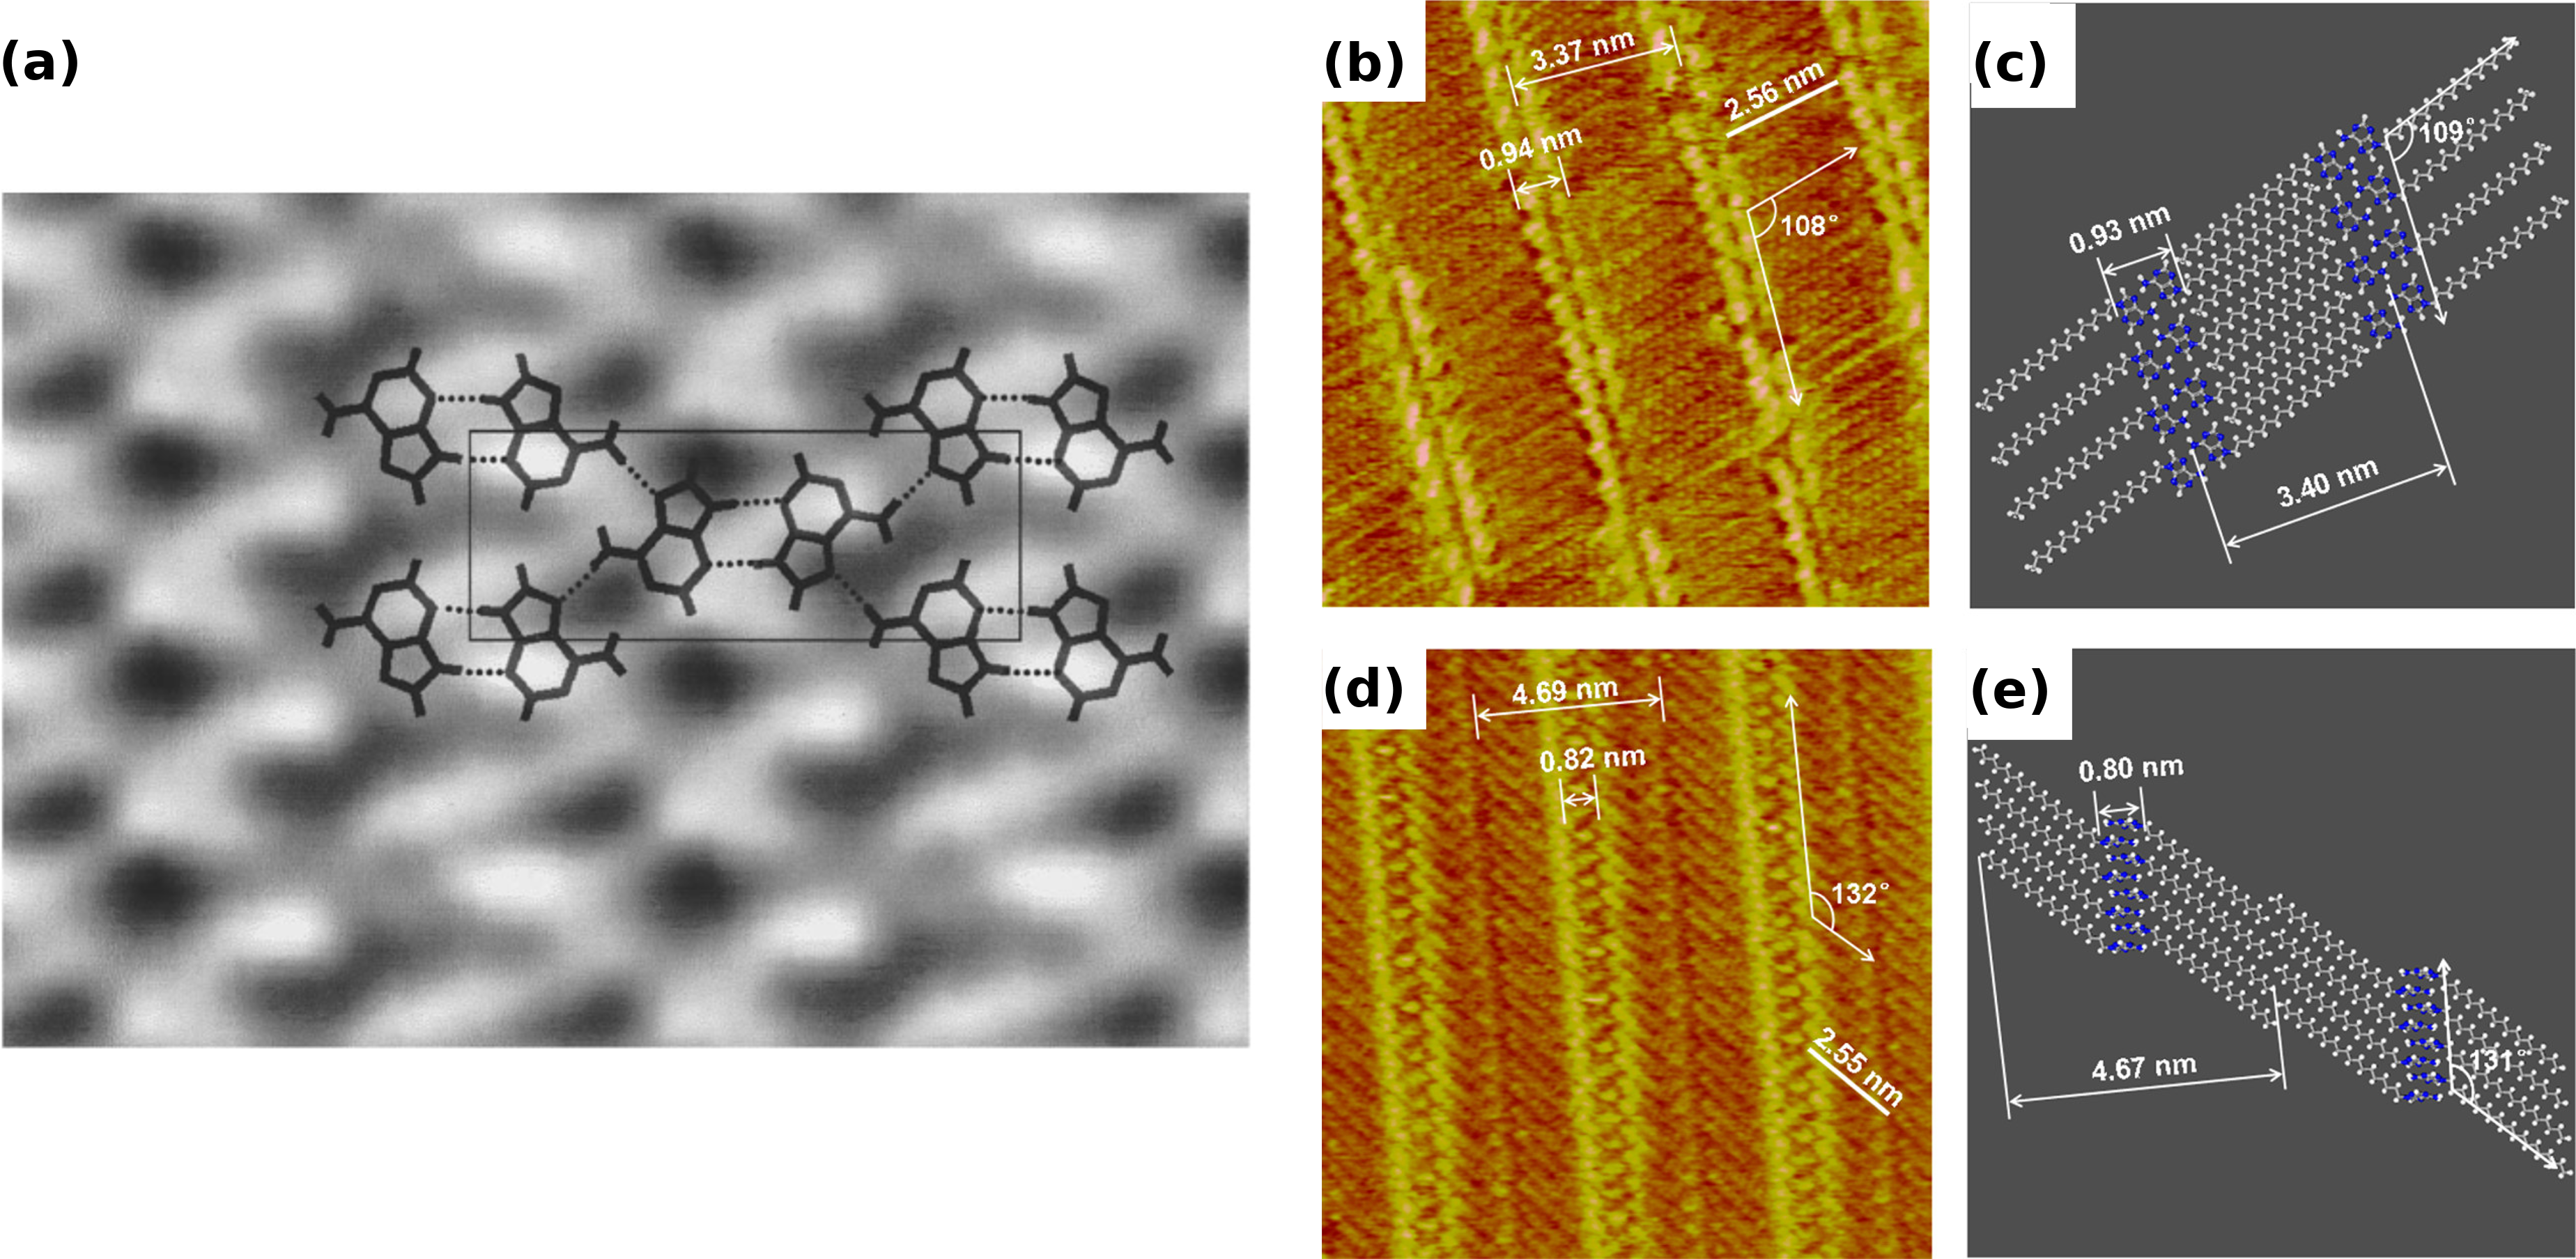
\includegraphics{Chapter2/Figures/Figure4.png}
    \caption[Representative structures depicting various aggregates formed in 0.50 and 0.75M simulations are presented. Probability distribution of the angle between the normal of the nucleobases ($\phi$) in the $\pi$-stacks are also presented]{Representative image from (a) 0.50 M and (b) 0.75 M simulation depicting the formation of aggregates. Probability distribution of the angle between the normal of the nucleobases ($\phi$) in the $\pi$-stacks from (c) 0.50 M and (d) 0.75 M simulations. Top and side views of the representative structures corresponding to the observed peaks are also presented.}
\end{figure}

On the basis of the analysis of the aggregate structures in solution we analyze the aggregate structures observed in the 0.50 and 0.75 M nucleobase - graphene simulations. We first analyze the formation of $\pi$-stacks before analyzing the formation of hydrogen-bonded structures. From Figure 4.2(d) and Figure 4.2(f), we observe that aggregate structures stabilized by $\pi$-$\pi$ interactions between the nucleobases are observed in regions (ii) 4.5 $\angstrom$ < d\textsubscript{Nuc-Graph} < 8.5 $\angstrom$ and (iii) d\textsubscript{Nuc-Graph} > 8.5 $\angstrom$. This is reflected in the $\theta$\textsubscript{Nuc-Graph} distribution. While the $\theta$\textsubscript{Nuc-Graph} exhibits a bimodal distribution for region (i) d\textsubscript{Nuc-Graph} $\leq$ 4.5 $\angstrom$, for regions (ii) and (iii) we observe a broad distribution spanning 0 - 180$\degree$ for both the 0.50 and 0.75 M simulations. The nucleobases in region (i) are stabilized by the $\pi$-$\pi$ interactions with the underlying graphene sheet, while in regions (ii) and (iii), they are stabilized by $\pi$-$\pi$ interactions among the nucleobases. The $\pi$-stacks are identified using the same geometric criterion of a distance cut off of 4.0 $\angstrom$ between the center of mass (d\textsubscript{COM-COM}) of the two nucleobases as described earlier. In Figures 4.6(a) and 4.6(b), we present the representative structures of the aggregates formed in regions (ii) and (iii). To identify the orientation of the nucleobases in the $\pi$-stacks we analyze the angle between the normal ($\phi$) of the nucleobases. The probability distribution corresponding to $\phi$ for all the identified $\pi$-stacked nucleobases is presented in Figures 4.6(c) and 4.6(d) for the 0.50 and 0.75 M nucleobase - graphene simulations. We observe that both the 0.50 and 0.75 M simulations favor a bimodal distribution. For 0.50 M, the peaks are centered around $\phi$ values of 9 and 171$\degree$, while for 0.75 M, the peaks are centered around 10 and 170$\degree$. Upon investigating the structural arrangement of the nucleobases, we observe that for 0.50 M simulations the antiparallel arrangement of the nucleobases is favored ($\phi$ = 171$\degree$), while for the 0.75 M simulations the slipped-stacked arrangement of the nucleobases is favored ($\phi$ = 10$\degree$). The arrangement and the relative orientations of the nucleobases in presented in Figures 4.6(c) and 4.6(d) for the 0.50 and 0.75 M simulations, respectively.

We next analyzed the simulation trajectories for the formation of hydrogen-bonded structures. The same hydrogen-bond criteria used earlier to identify the hydrogen-bonded structures in the nucleobase only simulations were followed. All hydrogen-bonded dimers were identified by enforcing a distance cutoff of 3.0 $\angstrom$ between the hydrogen-bond donor (D) and acceptor (A) and an angle cutoff of 20$\degree$ between the vectors directed through D-H and D-A bonds.  All hydrogen-bonded dimers with a probability of $\geq$50\% were classified as significant. We observed the formation of 15, 25, and 34 dimer pairs in the 0.25, 0.50, and 0.75 M nucleobase - graphene simulations, respectively. The probabilities of formation of stable dimeric assemblies were found to lie in the ranges of 54-88\%, 50-88\%, and 51-88\% for the 0.25, 0.50, and 0.75 M simulations and the corresponding plots are presented in Figure B.3 of the Appendix B. 
\begin{figure}
    \centering
    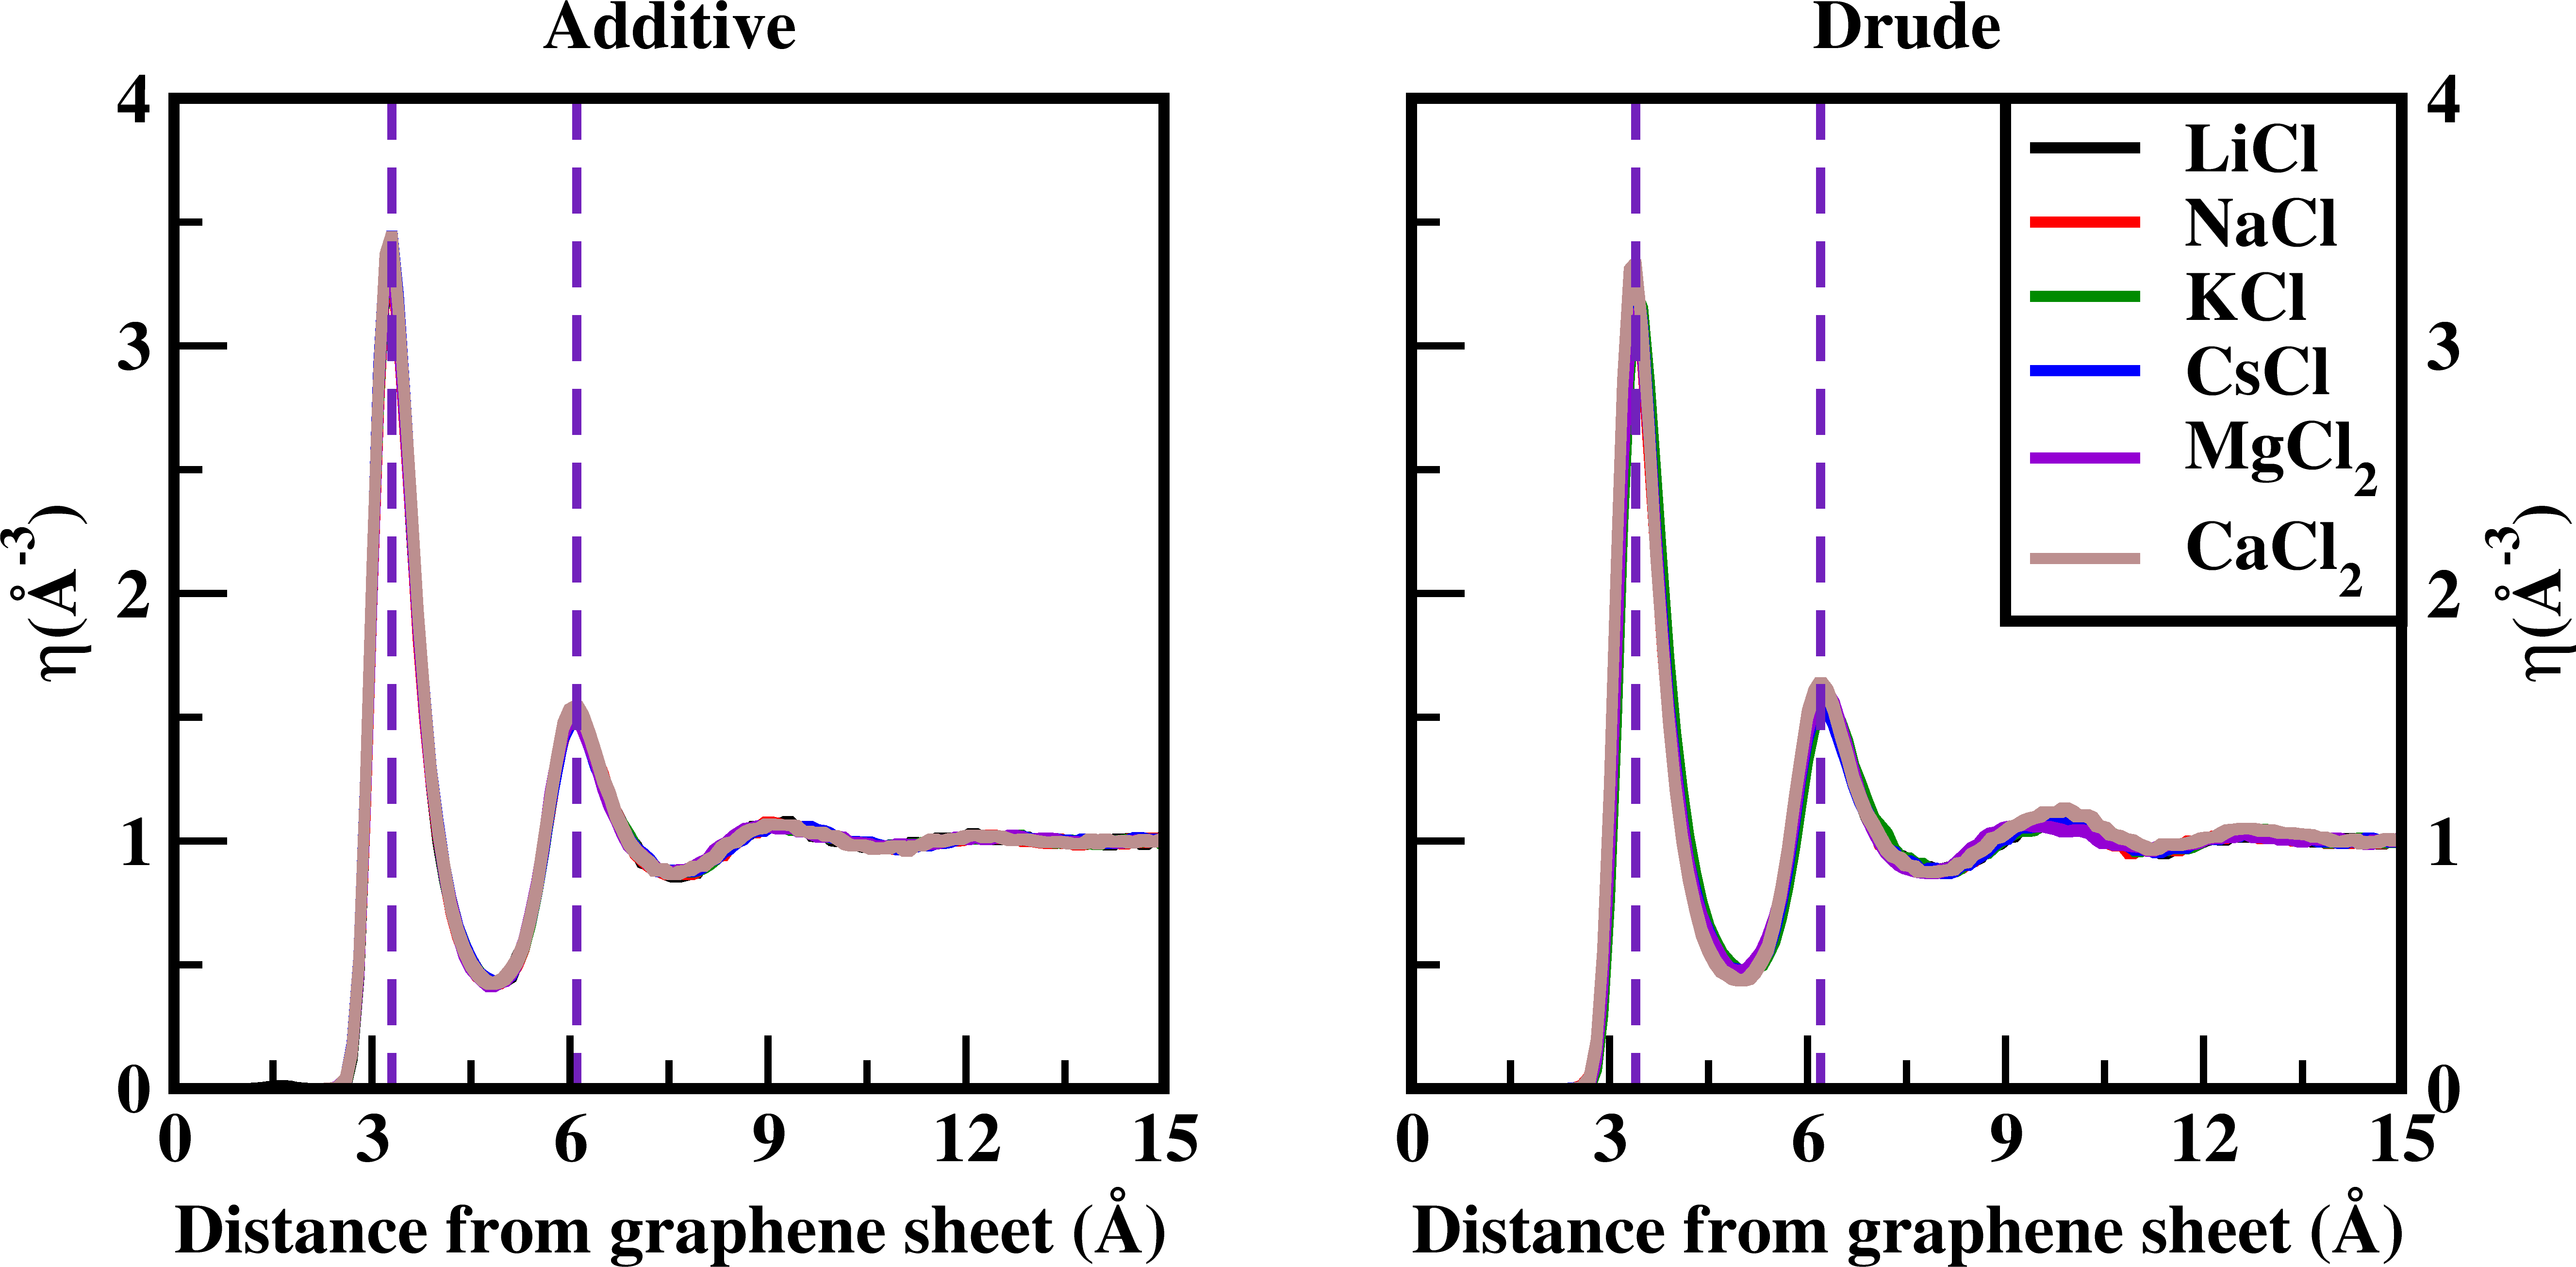
\includegraphics[width=\textwidth]{Chapter2/Figures/Figure5.png}
    \caption[Probability distribution of the angle between the normal ($\phi$) of the nucleobases involved in hydrogen-bond dimers. Representative images illustrating the arrangement of the nucleobases corresponding to the peaks in the distribution are also presented]{Probability distribution of the angle between the normal ($\phi$) of the nucleobases involved in hydrogen-bond dimers. Representative images illustrating the arrangement of the nucleobases corresponding to the peaks in the distribution are also presented. Atom numbering is also presented to illustrate the atoms involved in the hydrogen-bond. Dotted curves in the probability distribution correspond to hydrogen-bonded dimers observed in regions (ii) and (iii) of the 0.50 and 0.75 M simulations.}
\end{figure}

We classify the various dimeric assemblies based on the relative orientation of nucleobases within the dimer pairs. The relative orientation of nucleobase in hydrogen-bonded dimers were determined by calculating the angle between the normalized dipole moment vectors ($\phi$) in the identified hydrogen-bonded dimer pairs as discussed earlier for the solution simulation. The probability distribution of the relative orientation is presented in Figure 4.7. The atoms involved in various hydrogen-bonded dimers are presented in Table 4.1.
\begin{table}
    \centering
    \caption[Atoms involved in the hydrogen-bonds for the various structures observed in the nucleobase - graphene simulations]{Atoms involved in the hydrogen-bonds for the various structures observed in the nucleobase - graphene simulations}
    \begin{tabular}{cccc}
        \toprule
        Structure   &   Nucleobase I    &   Nucleobase II     &     Orientation \\ \midrule
        Cytosine\textsuperscript{I}\textsubscript{0.25M}    &   -NH\textsubscript{2}    &   C2(O)   &   72$\degree$ \\
        Cytosine\textsuperscript{II}\textsubscript{0.25M}   &   C2(O)   &   N1      &   115$\degree$    \\
        Cytosine\textsuperscript{III}\textsubscript{0.25M}  &   N3      &   C2(O)   &   173$\degree$    \\
                                                            &   C2(O)   &   N3      &   \\
        Cytosine\textsuperscript{I}\textsubscript{0.50M}    &   N3      &   -NH\textsubscript{2}    &   73$\degree$ \\
        Cytosine\textsuperscript{II}\textsubscript{0.50M}   &   -NH\textsubscript{2}    &   C2(O)   &   164$\degree$    \\
                                                            &   N3      &   N1      &   \\
        Cytosine\textsuperscript{I}\textsubscript{0.75M}    &   C2(O)   &   -NH\textsubscript{2}    &   60$\degree$ \\
        Cytosine\textsuperscript{II}\textsubscript{0.75M}   &   -NH\textsubscript{2}    &   C2(O)   &   166$\degree$    \\
                                                            &   N3      &   N1      &   \\  \bottomrule
    \end{tabular}
\end{table}

For the low (0.25 M) concentration limit, we observed the formation of three distinct dimer pairs, with average relative orientations of 72$\degree$ (Cytosine\textsuperscript{I}\textsubscript{0.25M}), 115$\degree$ (Cytosine\textsuperscript{II}\textsubscript{0.25M}), and 173$\degree$ (Cytosine\textsuperscript{III}\textsubscript{0.25M}). The dimer pairs with relative orientations of 72 and 115$\degree$ were observed to be transient structures with a single hydrogen bond between the interacting residues. Cytosine\textsuperscript{III}\textsubscript{0.25M} is stabilized by the formation of two symmetric hydrogen bonds between C2(O) and the N3 nitrogen of the interacting nucleobases. The Cytosine\textsuperscript{III}\textsubscript{0.25M} structure agrees with the kk2 structure previously reported by Fernandez et al.\supercite{gonzalez_competition_2017} and was also observed to be a part of C1-D(2) type ribbon structures for cytosine networks studied by Otero et al.\supercite{otero_elementary_2008} using STM imaging and DFT calculations. The dimer pairs Cytosine\textsuperscript{I}\textsubscript{0.25M} and Cytosine\textsuperscript{III}\textsubscript{0.25M} were previously observed by us from short simulations of cytosine nucleobases on graphene sheets.\supercite{h_polarization_2021} 

For intermediate (0.50 M) concentrations, we observe the formation of two distinct dimer pairs, with relative average orientations of 72$\degree$ (Cytosine\textsuperscript{I}\textsubscript{0.50M}) and 164$\degree$ (Cytosine\textsuperscript{II}\textsubscript{0.50M}). Cytosine\textsuperscript{I}\textsubscript{0.50M} appears as a transient structure with only one hydrogen-bond between the nucleobases. Cytosine\textsuperscript{II}\textsubscript{0.50M} was observed to be stabilized by two hydrogen bonds between the residues, with hydrogen bonds forming between the amino (-NH\textsubscript{2}) group and C2(O) and between the N3 and N1 nitrogen atoms. The structure assigned as Cytosine\textsuperscript{II}\textsubscript{0.50M} agrees with the structure kk1 previously reported by Fernandez et al. using REMPI spectroscopy and MM/DFT studies.\supercite{gonzalez_competition_2017} At high concentration (0.75M) limits, we observe the formation of two unique dimer pairs, with relative orientations of 60$\degree$ (Cytosine\textsuperscript{I}\textsubscript{0.75M}) and 166$\degree$ (Cytosine\textsuperscript{II}\textsubscript{0.75M}). The dimer pair with a relative average orientation of 166° (Cytosine\textsuperscript{II}\textsubscript{0.75M}) is structurally similar to the dimer pair Cytosine\textsuperscript{II}\textsubscript{0.50M}, with both structures being stabilized by two pairs of hydrogen bonds between the interacting nucleobases. Thus, from the nucleobase - graphene simulations we observe the formation of a dominant hydrogen-bonded dimer pair with relative orientation of $\phi$ $\geq$ 160$\degree$. This alludes to the effect of the underlying graphene sheet in stabilizing the interactions between the nucleobases by providing a solid support for the formation of planar/quasi-planar hydrogen-bonded dimers. However, we also note the gradual decrease in the probability of formation of planar/quasi-planar dimers with the increase in the concentration of nucleobases. In Figure 4.7, we also present the relative orientation of nucleobases in hydrogen-bonded dimers observed in the aggregate regions (ii) and (iii) from the 0.50 and 0.75 M simulations. We observe that the distribution is spread from 0 to 180$\degree$. Thus, at low concentrations we observe the formation of an ordered 2D assembly while at higher concentrations we see a shift toward complex 3D assembly of nucleobases. We notice that the hydrogen-bonded dimer distributions observed in the nucleobase - graphene simulations are very different from the distributions observed in the 0.60 M nucleobase only simulations. This is due to the differences in the binding energetics observed in the nucleobase - graphene and nucleobase - nucleobase systems. In our earlier study, we reported the $\pi$-stacking binding free energies between nucleobase - graphene and nucleobase - nucleobase to be -7.87 and 0.66 kcal/mol, respectively, while the nucleobase - nucleobase hydrogen-bonding free energy was estimated to be -2.03 kcal/mol. Thus, in a nucleobase - graphene system the nucleobases favor adsorption onto the graphene sheet followed by hydrogen-bonding between the nucleobases, while in a nucleobase-only system hydrogen-bonding is favored over formation of $\pi$-stacks, thereby resulting in the observed differences in the hydrogen-bonding patterns.
\begin{figure}
    \centering
    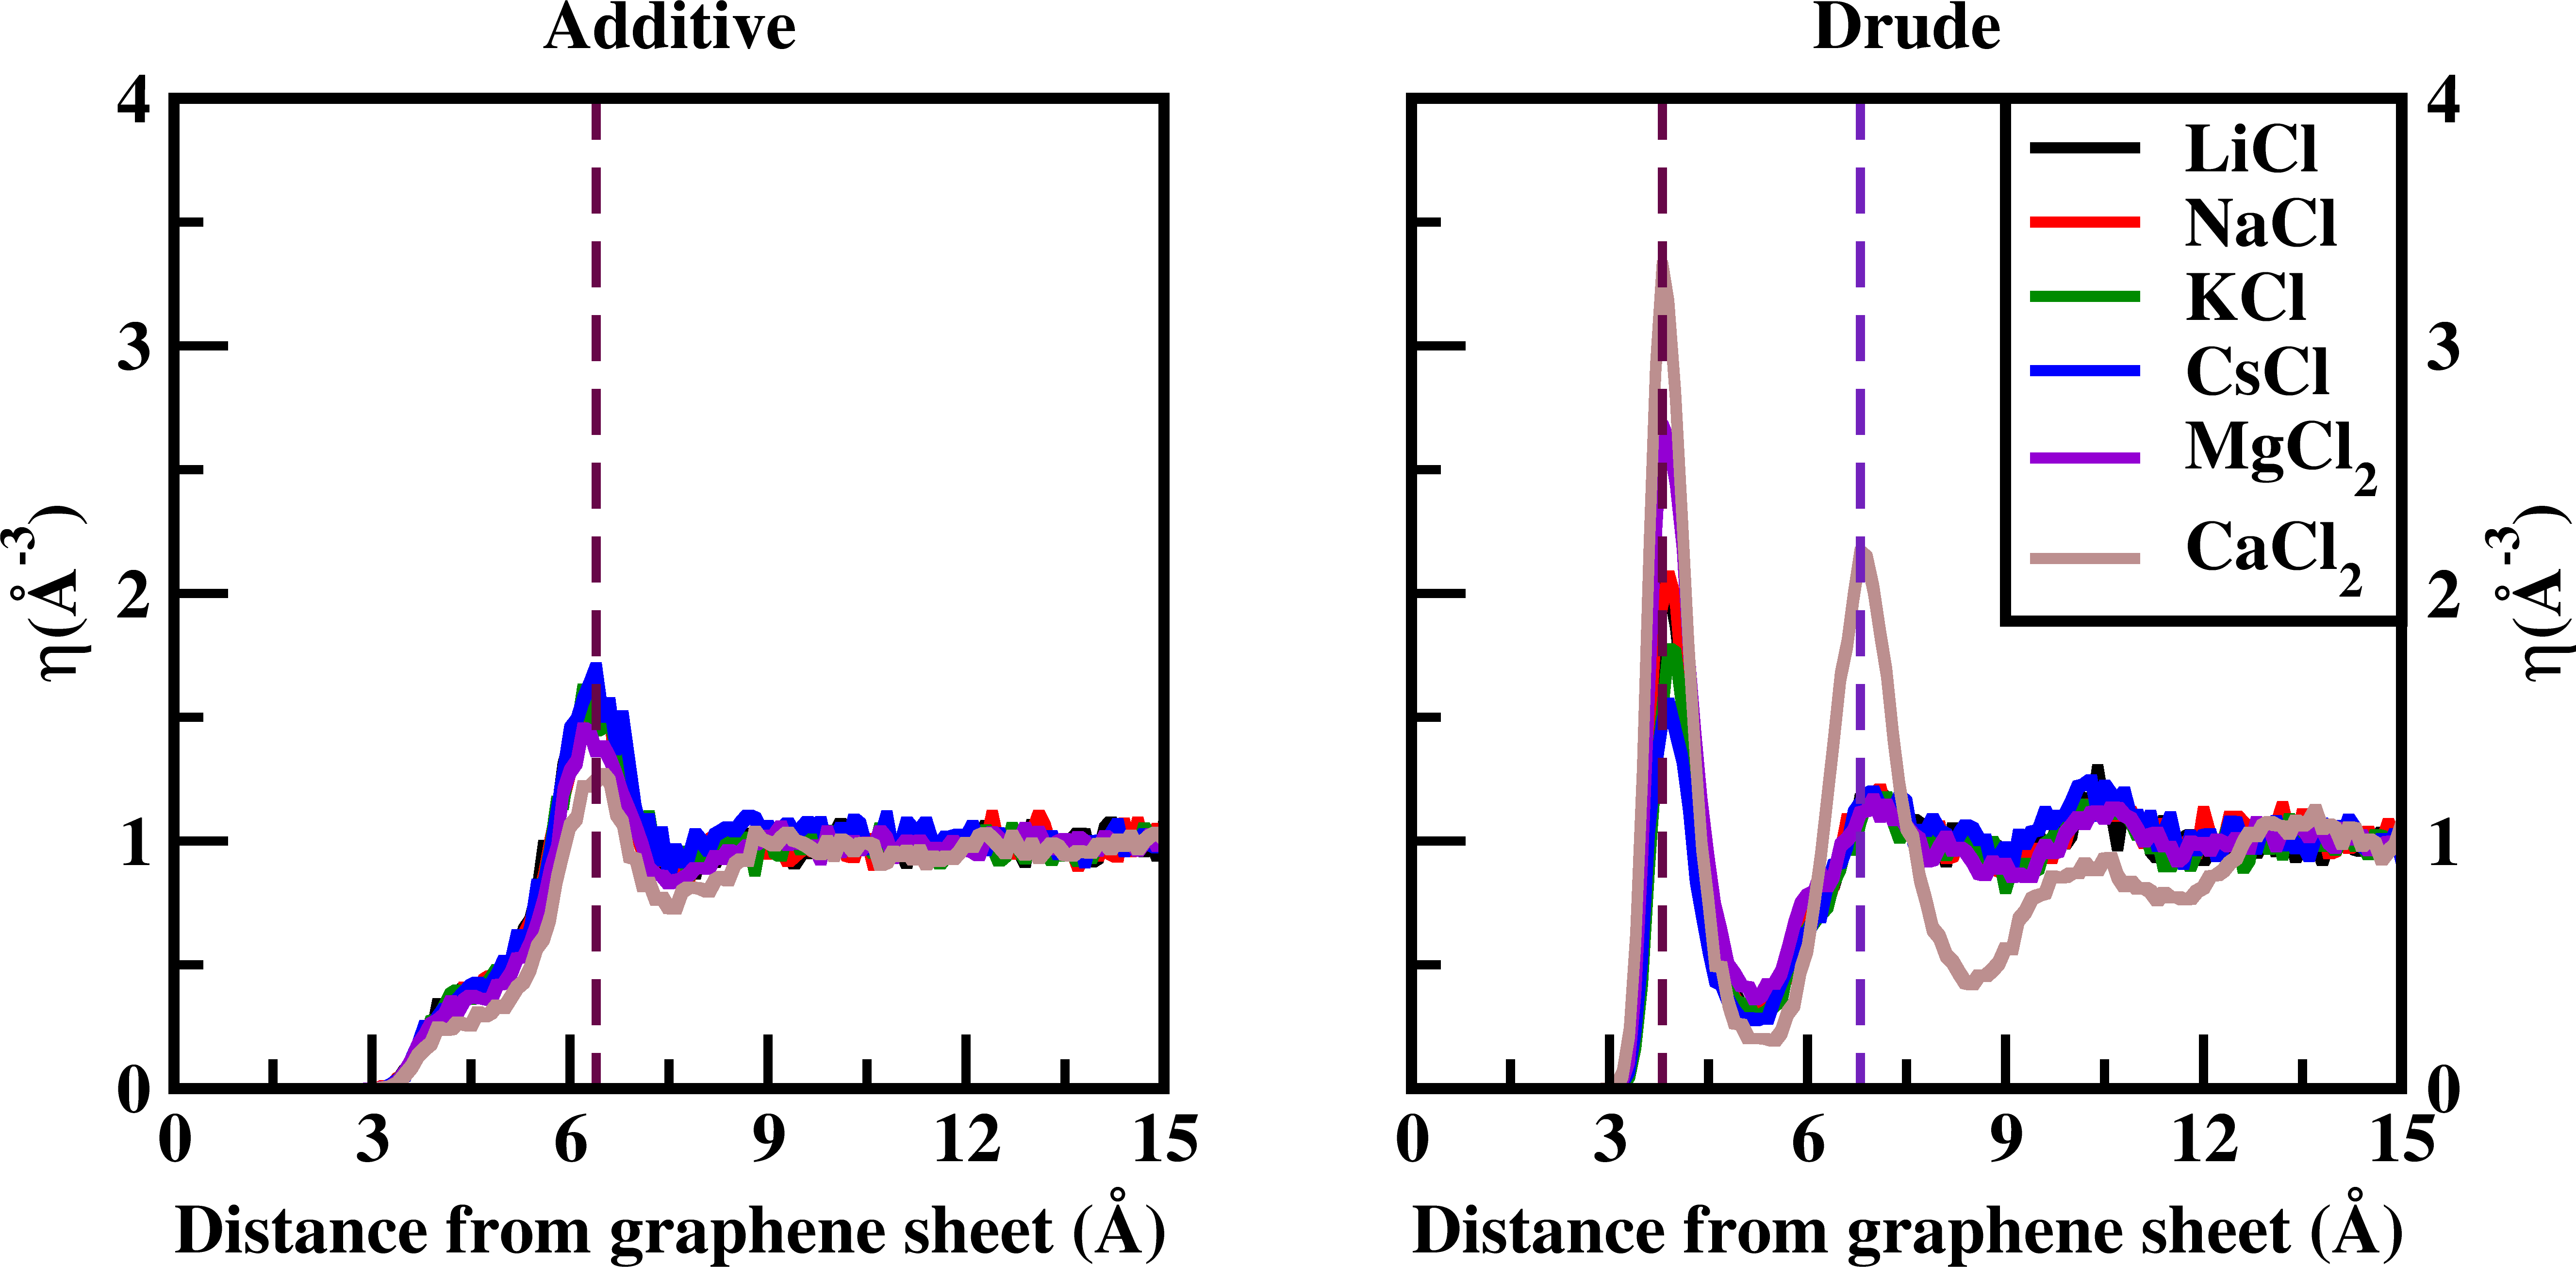
\includegraphics[width=\textwidth]{Chapter2/Figures/Figure6.png}
    \caption[Time series of the center-of-mass to center-of-mass descriptor used to identify the nucleobase assemblies observed in 0.25 M simulations. Representative structures depicting the 2D network corresponding to different regions of the d\textsubscript{COM-COM} time series. Representative structures of nucleobase assemblies in 0.50 M and 0.75 M simulations]{(a) Time series of the center-of-mass to center-of-mass descriptor used to identify the nucleobase assemblies observed in 0.25 M simulations. Representative structures depicting the 2D network corresponding to (b) region-I, (c) region-II, and (d) region-III of the d\textsubscript{COM-COM} time series. Representative structures of nucleobase assemblies in (e) 0.50 M and (f) 0.75 M simulations. The simulation cell is indicated in yellow color and periodic images of the cell are colored green. (b-d) Nucleobases used in the center-of-mass metric are in red (3) and orange (21). All other nucleobases are colored blue. (e) and (f) Nucleobases are color-coded with respect to the distance from the graphene sheet. Nucleobases in regions (i) (d\textsubscript{Nuc-Graph} < 4.5 $\angstrom$), (ii) (4.5 $\angstrom$ < d\textsubscript{Nuc-Graph} < 8.5 $\angstrom$), and (iii) (d\textsubscript{Nuc-Graph} > 8.5 $\angstrom$) are presented in red, blue, and green, respectively.}
\end{figure}

Cytosine nucleobases are known to form hydrogen-bonded assemblies on 2D supports like Au(111),\supercite{kelly_understanding_2008, otero_elementary_2008} Cu(111), and HOPG.\supercite{xu_directional_2021} Having analyzed the relative orientations of nucleobases in the hydrogen-bonded dimers observed in the nucleobase - graphene sheet simulations, we next analyze the formation of two-dimensional network structures in these simulations. Inspection of the simulation trajectory reveals the formation 2D assemblies for the low concentration limit of 0.25 M, while 3D structures are observed for 0.75 M. This is also visible in the representative images presented in Figure 4.2. To identify the network structures, we employed the distance between the center of mass of two selected nucleobases (d\textsubscript{COM-COM}) as the metric to analyze the formation of such networks. The nucleobases were chosen in such a fashion that the COM-COM distance between them was able to accurately capture the dynamics of the 2D network under consideration. For the 0.25 M simulation, we employed the COM-COM distance between the 3\textsuperscript{rd} and 21\textsuperscript{st} nucleobases to describe the dynamics of the network. We present the d\textsubscript{COM-COM} time series corresponding to the selection in Figure 4.8(a). From the d\textsubscript{COM-COM} time series, we observe three distinct time series blocks wherein separate network structures exist. We denote the three blocks as follows: Region-I, corresponding to the initial 50 ns of the analyzed trajectory; Region-II, corresponding to the 50-300 ns window, and Region-III, corresponding to the last 200 ns of trajectory. We observe that for the initial 50 ns of the analyzed trajectory, the COM-COM distance oscillates around an average value of 20 $\angstrom$. In this region, we observe the formation of two different clusters which are in constant motion. This is depicted in the representative structure presented in Figure 4.8(b). After the initial 50 ns, the COM-COM distance quickly settles to an average distance of 25 $\angstrom$. This distribution persists to the last 200 ns. In this region we observe the formation of a periodic zigzag ribbon structure that spans across the periodic boundary conditions of the simulation cell. This is illustrated by the representative structure presented in Figure 4.8(c). Beyond 300 ns, we again observe fluctuations in the distance distribution. The periodic network structure breaks away and leads to the formation of island structures, as illustrated by the representative structure presented in Figure 4.8(d). Both the long network structures as well as the island structures have been observed in experimental studies and by STM imaging of cytosine nucleobases adsorbed on metal surfaces such as Au(111).\supercite{kelly_understanding_2008,wandlowski_structure_1996,iakhnenko_adsorption_2013,hsu_stm_2021}

Upon increasing the concentration of the nucleobases, we observe an increase in the $\pi$-$\pi$ interaction between the nucleobases, as the monolayer assembly is replaced by multiple layers. The 2D periodic network structure is lost and is replaced by a 3D arrangement of nucleobases favored by interaction between $\pi$-stacks. In Figure 4.8(e), we present the representative structure of the clustered assembly of the nucleobases. The various stacks are presented to highlight the formation of 3D layered structures. For the 0.50 M simulations, the nucleobases are dispersed in various layers. Upon increasing the concentration to 0.75 M, we saturate the graphene sheet with nucleobases, which results in the formation of a pseudoperiodic assembly of the nucleobases in addition to the formation of 3D layered structures. This is reflected in the representative structure presented in Figure 4.8(f).
\begin{figure}
    \centering
    \includegraphics[width=\textwidth]{Chapter2/Figures/Figure7.png}
    \caption[Hydrogen-bonded networks observed in the periodic structure in monolayer assemblies stabilized by the two specific patterns, linear zigzag structures and circular hexagonal arrangement. HR-STM images from experimental reports are also presented]{(a) Hydrogen-bonded networks observed in the periodic structure in monolayer assemblies stabilized by the two specific patterns, linear zigzag structures and circular hexagonal arrangement. (b) HR-STM image (5 × 5 nm2, scale bar, 1 nm) of pure cytosine at the 1-octanol/HOPG interface. Image adapted with permission from ref. \supercite{xu_coadsorption_2006}. Copyright 2022 American Chemical Society. (c) HR-STM for self-assembled domain of melamine-cytosine coassembly. (d) Dmol3 calculated structure of the proposed hexagonal arrangement with six cytosine nucleobases surrounding a central melamine molecule. (c) and (d) Adapted from ref. \supercite{zhao_investigating_2016} under the terms of the Creative Commons Attribution 4.0 International License (http://creativecommons.org/licenses/by/4.0/).}
\end{figure}

In Figure 4.9(a), we present a detailed view of the hydrogen-bonded assemblies that stabilize the periodic monolayer assembly. We notice the formation of a central node which comprises of seven nucleobases arranged in a circular hexagonal fashion. These nodes are connected to an arm-type arrangement that is facilitated by the zigzag linear arrangement of the cytosine nucleobases. It is noted that these assemblies are stabilized by both symmetric and asymmetric hydrogen-bonds between the nucleobases. These arrangements have been have observed for cytosine nucleobases adsorbed on liquid/solid 1-octanol/HOPG interfaces.\supercite{zhao_investigating_2016,xu_coadsorption_2006} Pure cytosine adsorbed at the 1-octanol/HOPG interface is found to be arranged in the linear zigzag fashion. This was investigated by Xu et al. using high-resolution STM (HR-STM). In Figure 4.9(b), we reproduce the high-resolution STM image of pure cytosine adsorbed at the 1-octanol/HOPG interface, wherein the zigzag arrangement of the bases is clearly observed.\supercite{xu_coadsorption_2006} Zhao et al. studied the coadsorption of melamine and cytosine at the 1-octanol/HOPG interface using HR-STM. They found the formation of distorted hexagonal molecular-assembled island structures. We reproduce the HR-STM images obtained by Zhao et al. in Figure 4.9(c).\supercite{zhao_investigating_2016} Using DFT calculations, they ascribed the hexagonal assembly to a melamine molecule surrounded by six cytosine molecules. In Figure 4.9(d), we reproduce the calculated structure proposed by Zhao et al.\supercite{zhao_investigating_2016} We observe that the circular node structure observed by us, wherein a central cytosine is surrounded by six other cytosine nucleobases, is similar to the arrangement of the central melamine surrounded by six cytosine nucleobases. This direct correlation of our simulations with experimentally realized molecular arrangements highlights the strength of polarizable simulations in capturing the self-assembly of nucleobases on 2D graphene support.
\section{Conclusions}
In conclusion, we have investigated the influence of concentration on the self-assembly behavior of nucleobases on a 2D graphene support. The study sheds light on the dynamics of multilayered self-assemblies, hitherto unexplored in the literature, by the inclusion of polarization into simulations. The accurate description of the various interactions forces (Hydrogen-bonded and $\pi$-stacking) allowed us to study the evolution of the dynamics of the system.  At low concentrations (0.25 M), $\pi$-stacking interactions between the graphene surface and nucleobases were found to drive the dynamics of the system. At an intermediate concentration (0.50 M), we observe competition between graphene - nucleobases $\pi$-stacking interactions and nucleobase - nucleobase interactions, leading to the formation of multilayered assemblies. This resulted in the formation of a 3D aggregate structure tethered to the graphene sheet. At a high concentration limit (0.75 M), which is closer to the surface loading limit, our study captures the formation of pseudo-2D assemblies of the nucleobases on the graphene sheet that support 3D aggregate assemblies. This reflects a transition toward glassy networks. These observations are consistent with the experimental observation of cytosine nucleobases adsorbed on 1-octanol/HOPG solid-liquid interfaces and Au(111) surfaces,\supercite{kelly_understanding_2008, wandlowski_structure_1996, zhao_investigating_2016, xu_coadsorption_2006} where such glassy networks were observed via HR-STM imaging. In conclusion, we show that a generalized polarizable FF can accurately capture the formation of self-assembled structures, without the need for specific interaction potentials. We believe that this study would pave the way for further studies on small-molecule assemblies with applications in nanopatterning and tailored self-assemblies. The study will also serve as a benchmark for the applicability of polarizable simulations in capturing solid-liquid interfacial phenomenon.